\begin{problemAllDefault}{Електричка}

На кожному вагоні електрички є табличка, на якій фарбою написано його номер. Вагони занумеровані натуральними числами\nolinebreak[1] 1,\nolinebreak[2] 2,~\dots,\nolinebreak[2] $N$ (крайній вагон має номер~1, сусідній з ним\nolinebreak[3] --- номер~2, і~т.~д., до\nolinebreak[3] крайнього з протилежного боку вагону, який має номер~$N$). Електричка має кабіни з обох боків, і\nolinebreak[3] може поїхати хоч\nolinebreak[2] \mbox{1-им} вагоном уперед, хоч\nolinebreak[3] \mbox{$N$-им}.

\ifnum\pdfoutput>0
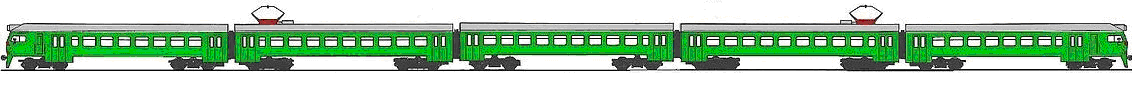
\includegraphics[width=\textwidth,keepaspectratio=true]{elTrain.png}
\else
\fbox{\colorbox{yellow}{Run not latex but pdflatex to insert picture}}
\ifnum\number\month > 6 \ERROR \fbox{Run not latex but pdflatex to insert picture}\fi
\fi

Під час прибуття електрички на платформу, Вітя помітив, що ${(i{-}1)}$ штук вагонів електрички проїхали мимо нього, а\nolinebreak[2] \mbox{$i$-й} по\nolinebreak[2] порядку зупинився якраз навпроти. Ще\nolinebreak[2] він помітив, що\nolinebreak[2] на\nolinebreak[2] табличці цього вагона написаний номер~$j$. Ще\nolinebreak[2] він точно знає (і\nolinebreak[2] ці\nolinebreak[2] знання відповідають дійсності), що\nolinebreak[2] електрички ніколи не\nolinebreak[3] бувають ні\nolinebreak[3] коротшими 4~вагонів, ні\nolinebreak[3] довшими 12~вагонів. Вітя хоче визначити, скільки всього вагонів у\nolinebreak[2] електричці. Напишіть програму, яка або\nolinebreak[2] знаходитиме цю кількість, або\nolinebreak[2] повідомлятиме, що без\nolinebreak[1] додаткової інформації це\nolinebreak[1] зробити неможливо.

\InputFile
Програма має прочитати зі\nolinebreak[3] стандартного входу (клавіатури) два цілі числ\'{а} $i$ та~$j$, розділені пропуском. ${2{\<}i{\<}12}$, ${2{\<}j{\<}12}$, ч\'{и}сла гарантовано задовольняють всі вищезгадані обмеження.

\OutputFile
Виведіть на стандартний вихід (екран) одне число\nolinebreak[3] --- кількість вагонів у\nolinebreak[3] електричці. Якщо однозначно визначити кількість вагонів неможливо, виведіть замість кількості число~\texttt{0}.

\Example
\begin{exampleSimple}{3em}{3em}%
\exmp{4 2}{5}%
\end{exampleSimple}

\end{problemAllDefault}
